\documentclass[unicode]{beamer}
\usepackage[T2A]{fontenc}
\usepackage[utf8]{inputenc}
\usepackage[russian]{babel}
\usepackage{cmap}
\usepackage{amssymb,amsfonts,amsmath,mathtext}
\usepackage{graphicx}
% XeTeX packages
\usepackage[cm-default]{fontspec} % or install lmodern and remove cm-default opt
\usepackage{xunicode} % some extra unicode support
\usepackage{xltxtra} % \XeLaTeX macro
\defaultfontfeatures{Scale=MatchLowercase,Mapping=tex-text}

\setromanfont{Charis SIL}
\setsansfont{Charis SIL}
\setmonofont{Charis SIL}

\usepackage{geometry}
\geometry{left=0mm}
\geometry{right=0mm}
\geometry{top=0cm}
\geometry{bottom=0cm}

\usepackage{array}

\setbeamerfont{institute}{size=\normalsize}
\graphicspath{{images/}}
\usetheme{CambridgeUS}
\useoutertheme{shadow}
\useinnertheme{rounded}
\usecolortheme{beaver}
\usefonttheme{professionalfonts}


\title[Разработка расширений для системы управления проектами Redmine]{
Разработка расширений для системы управления проектами Redmine
}
\author[Кандауров О.\,В.]{Студент 5-го курса О. Кандауров}
\institute{
Научный руководитель: ст. преподаватель Парамонов~И.\,В.
}
\date{}
\begin{document}
\maketitle

\begin{frame}
\transwipe[direction=90]
\frametitle{Системы управления проектами}
\begin{columns}
\begin{column}{0.45\textwidth}
\begin{block}{Функциональность}
\begin{itemize}
  \item Планирование
  \item Постановка задач
  \item Оценка и разработка
  \item Управление бюджетом
  \item Распределение ресурсов
  \item Взаимодействие
  \item Документирование
\end{itemize}
\end{block}
\end{column}
\begin{column}{0.55\textwidth}
\centerline{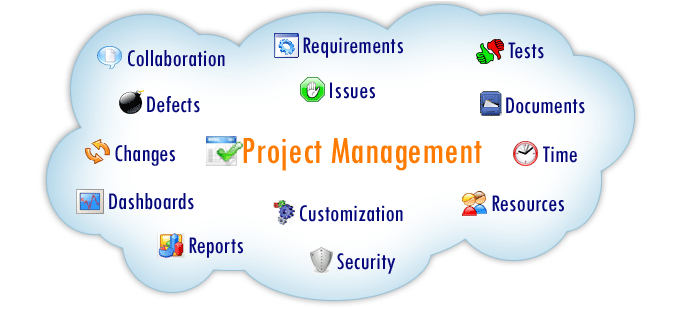
\includegraphics[width=1\textwidth]{project-management-software.png}}
\end{column}
\end{columns}
\end{frame}

\begin{frame}
\transwipe[direction=90]
\frametitle{Redmine}
\begin{block}{}
\small
\begin{itemize}
   \item Работает в браузере
   \item Открытые исходные коды
   \item Богатая функциональность
   \item Расширяемость
   \item Активно развивается
\end{itemize}
\end{block}
\centerline{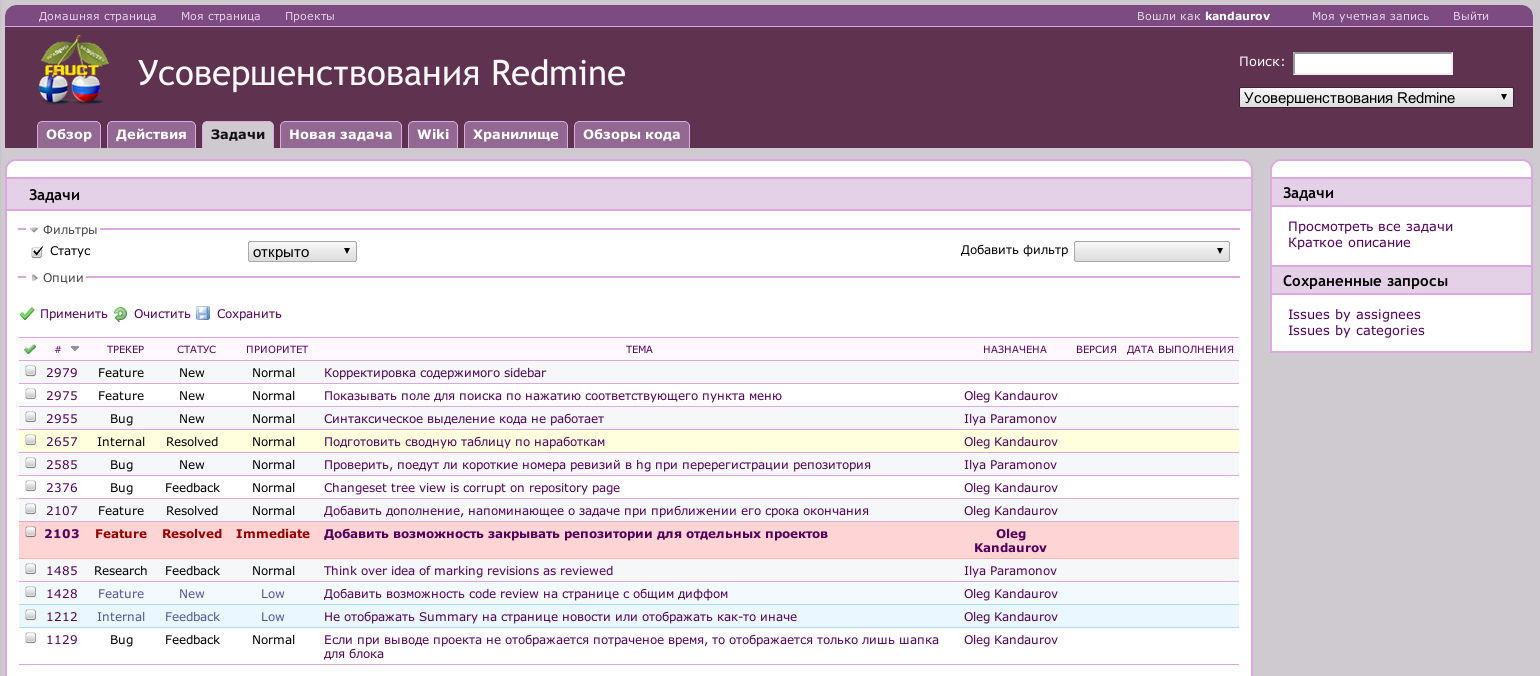
\includegraphics[width=1\textwidth]{redmine-issues.png}}
\end{frame}

\begin{frame}
\transwipe[direction=90]
\frametitle{Постановка задачи}
\begin{block}{}
\begin{itemize}
  \item Реализовать дополнительный функционал
  \begin{itemize}
    \item Ограничения доступа к репозиториям
    \item Ограничение доступа к вики-страницам
    \item Рассылка уведомлений о приближающихся и просроченных задачах
    \item Изображения-ссылки в боковой панели
    \item Установка статуса задачи на `Resolved` через сообщение коммита
  \end{itemize}
  \item Внесение улучшений
  \begin{itemize}
    \item В механизм позиционирования всплывающего календаря
    \item В систему навигации между страницами просмотра изменений
  \end{itemize}
  \item Разработать механизм, упрощающий поддержку наработок
\end{itemize}
\end{block}
\end{frame}


\begin{frame}
\transwipe[direction=90]
\frametitle{Способы внесения изменений}
\begin{tabular}{ >{\centering\arraybackslash}m{0.3\textwidth}  >{\centering\arraybackslash}m{0.3\textwidth}
>{\centering\arraybackslash}m{0.3\textwidth}}

&
\includegraphics[width=1cm]{Ruby_logo.pdf}&
\includegraphics[width=1cm]{patch-management.jpg}\\
& Система плагинов Redmine & Механизм патчей\\
&&\\
\hline
\color{blue}{Сложность разработки} & Высокая & \color{red}{Низкая} \\
\hline
\color{blue}{Спектр решаемых задач} & Ограниченный & \color{red}{Максимальный}\\
\hline
\color{blue}{Устойчивость к обновлениям системы} & \color{red}{Высокая} & Низкая \\
\hline
\color{blue}{Стоимость внесения изменений} & Высокая & \color{red}{Средняя} \\
\hline
\color{blue}{Удобство распространения} & \color{red}{Высокое} & Низкое \\
\hline
\end{tabular}
\end{frame}

\begin{frame}
\transwipe[direction=90]
\frametitle{Mercurial Queues}
\centerline{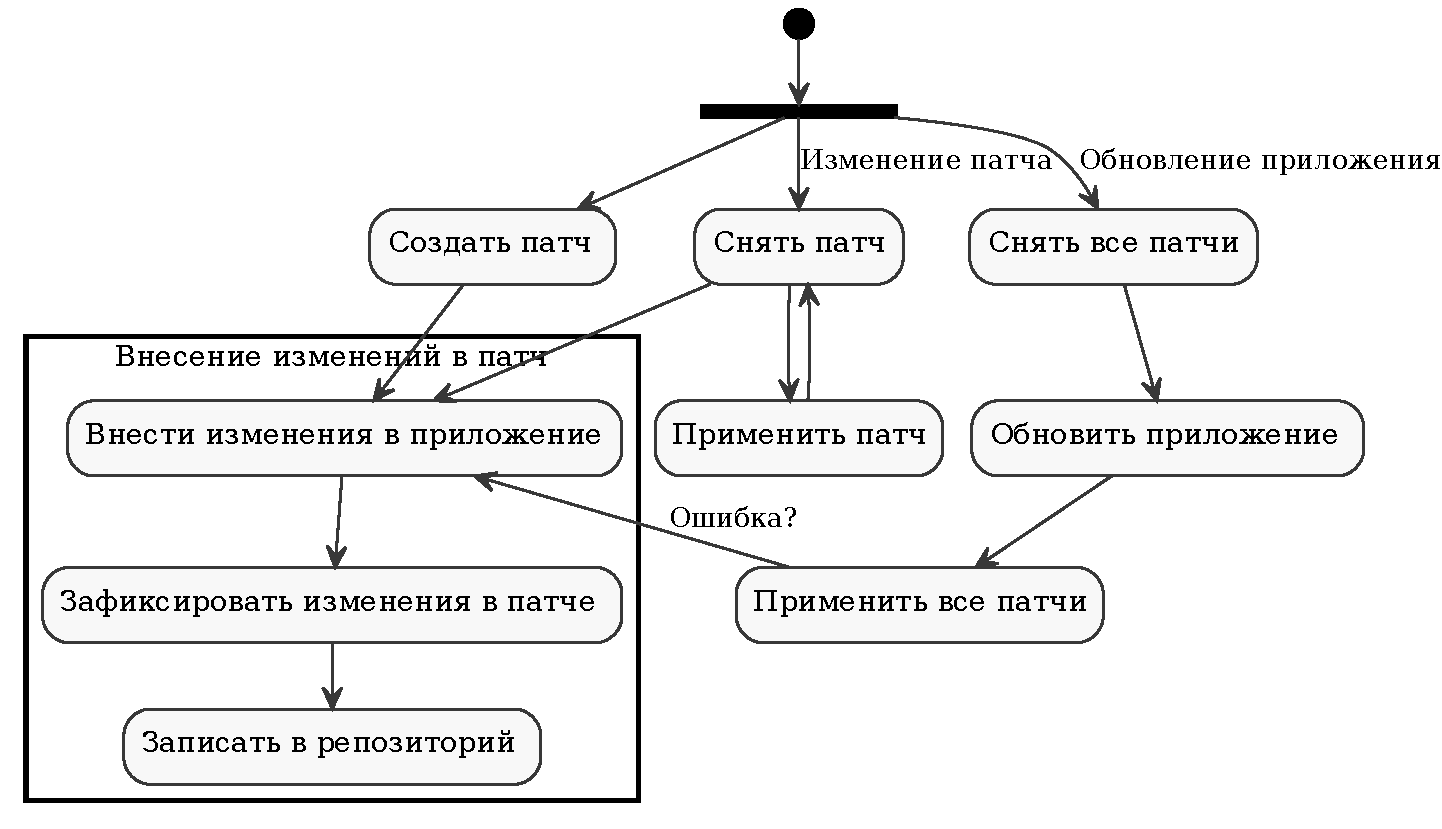
\includegraphics[width=1\textwidth]{mq-workflow.pdf}}
\end{frame}

\begin{frame}
\transwipe[direction=90]
\frametitle{Плагин для рассылки уведомлений}
\begin{columns}
\begin{column}{0.6\textwidth}
\begin{block}{Функционал}
\begin{itemize}
  \item Уведомление о задачах, срок исполнения которых истекает (конфигурируемое)
  \item Уведомление о просроченных задачах (принудительное)
  \item Формат: общий список просроченных задач, отсортированных по проектам и по "степени просроченности"
\end{itemize}
\end{block}
\end{column}
\begin{column}{0.4\textwidth}
\centerline{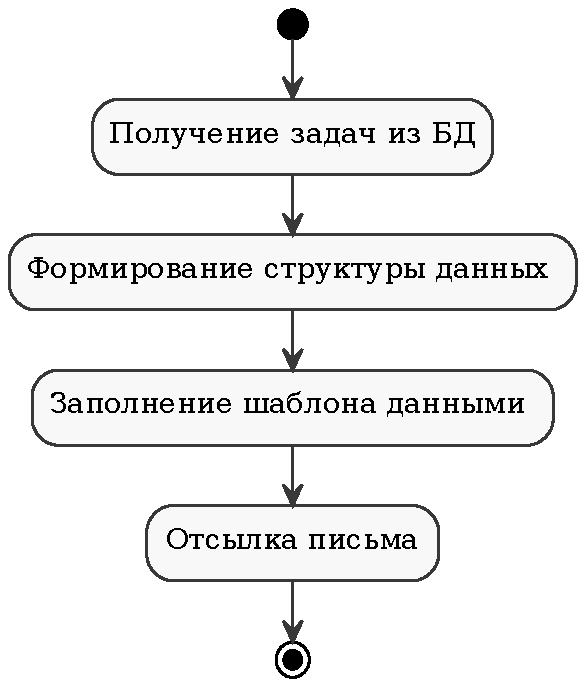
\includegraphics[width=1\textwidth]{reminder-plugin.pdf}}
\end{column}
\end{columns}
\end{frame}


\begin{frame}
\transwipe[direction=90]
\frametitle{Передача наработок}
\begin{columns}
\begin{column}{0.6\textwidth}
\begin{block}{}
\begin{itemize} 
  \item Привлечение пользователей
  \begin{itemize}
  	\item Отзывы/Предложения
  	\item Тестирование
  \end{itemize}
  \item Привлечение сторонних разработчиков	
  \begin{itemize}
  \item Патчи
  \end{itemize}  
\end{itemize}
\end{block}
\end{column}
\begin{column}{0.4\textwidth}
\centerline{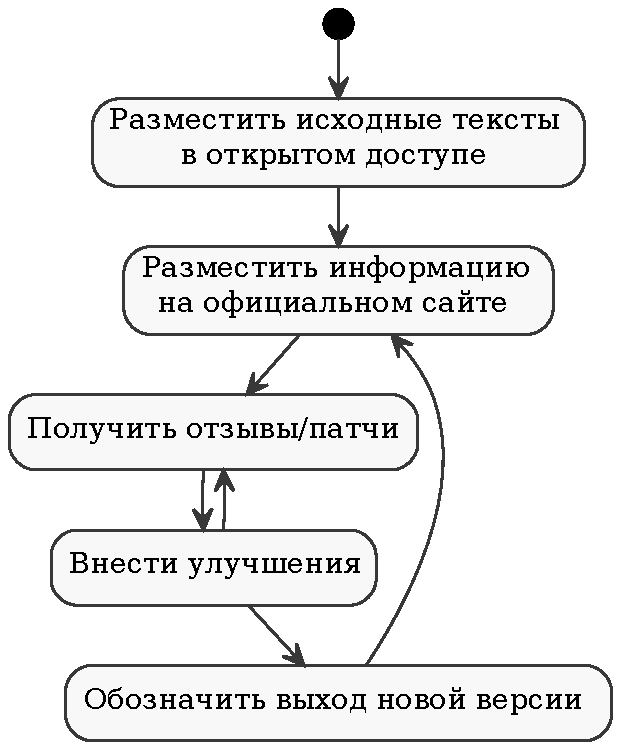
\includegraphics[width=1\textwidth]{opensource-feedback.pdf}}
\end{column}
\end{columns}
\end{frame}


\begin{frame}
\transwipe[direction=90]
\frametitle{Результаты}
\begin{block}{Достигнутые результаты}
\begin{itemize}
  \item Добавлен новый функционал  (разработано 4 плагина)
  \item Внесены улучшения (более 15 патчей)
  \item Внедрена система управления патчами (4 успешных обновления)
  \item Наработки выложены в открытый доступ
\end{itemize}
\end{block}
\end{frame}

\begin{frame}
\transwipe[direction=90]
\frametitle{}
\centerline{\large{Cпасибо за внимание!}}
\hspace{2cm}
\centerline{\huge{Вопросы?}}
\end{frame}


\end{document}